% Prof. Dr. Ausberto S. Castro Vera
% UENF - CCT - LCMAT - Curso de Ci\^{e}ncia da Computa\c{c}\~{a}o
% Campos, RJ,  2021
% Disciplina: Paradigmas de Linguagens de Programa\c{c}\~{a}o
%

\chapter{Ferramentas}
Nesse capítulo apresentamos as três principais ferramentas do ecossistema Julia são os ambientes: VScode, JupyterNotebook e Juno. 
Ocupam lugar de destaque no próprio site da linguagem (Fig \ref{julia_editors_site}), além de ocuparem as primeiras posições no \href{https://julialang.org/blog/2021/08/julia-user-developer-survey/}{questionário anual de 2021} que coletou respostas de 2 660 usuários da linguagem (Fig \ref{julia_editors_survey}). 

   \begin{figure}[H]
    \begin{center}
        \caption{Editores preferidos dos usuários de Julia em 2021} \label{julia_editors_survey}
        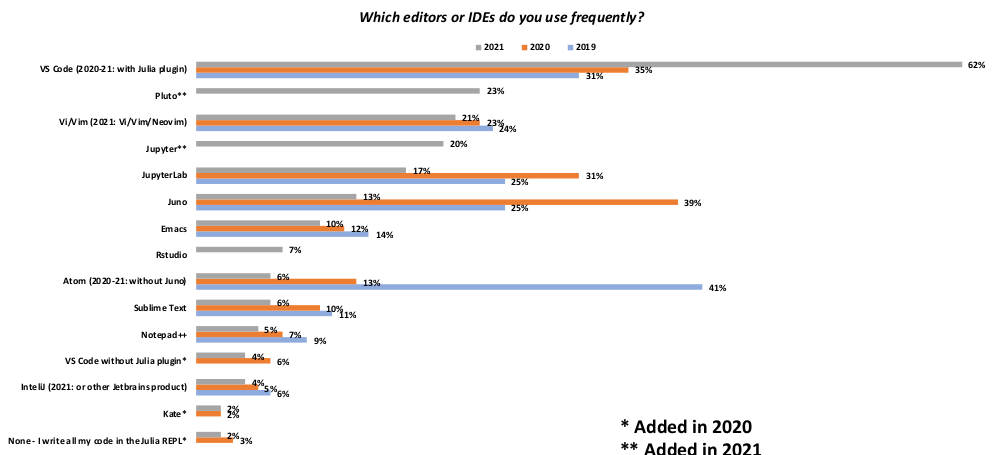
\includegraphics[width=12cm]{aplicacoes/Editores e IDEs.png} \\
        {\tiny \sf Fonte: https://julialang.org/blog/2021/08/julia-user-developer-survey }
    \end{center}
   \end{figure} 

   \begin{figure}[H]
    \begin{center}
        \caption{Editores e IDEs destacadas no site da linguagem} \label{julia_editors_site}
        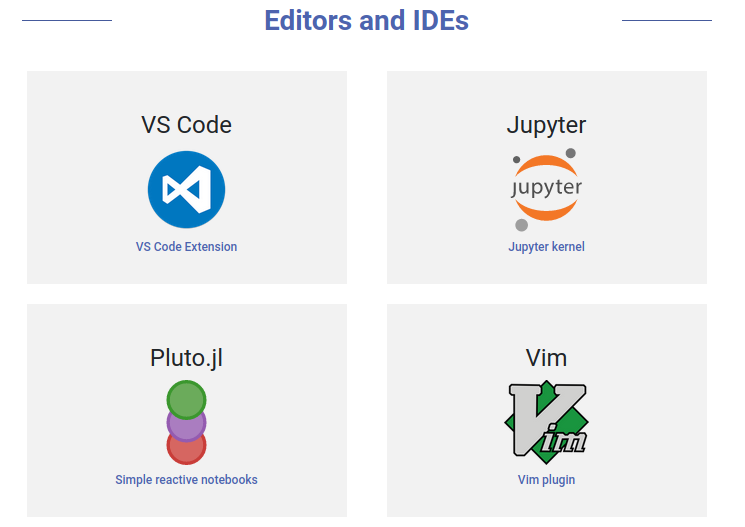
\includegraphics[width=12cm]{aplicacoes/Editors_IDEs_site.png} \\
        {\tiny \sf Fonte: https://julialang.org/}
    \end{center}
   \end{figure} 

\section{Visual Studio Code}

\section{Jupyter Notebook}

\section{Juno}
